\textbf{\underline{OZ 7 - Inductantie - Oefening 3:}}
\vspace{0.5cm}

Beschouw een circuit waarbij $ \mathcal{E} = 6,00 $ V, $ L = 8,00 $ mH, en $ R = 4,00 \ \Omega $.

\vspace{0.3cm}
\begin{minipage}{.75\textwidth}
    \begin{enumerate}[(a)]
        \item Wat is de inductieve tijdsconstante $ \tau $ van het circuit?
        \item Bereken de stroom in het circuit 250 $ \mu $s nadat de schakelaar gesloten werd.
        \item Wat is de uiteindelijke (steady-state) stroom?
        \item Hoe lang duurt het voordat de stroom 80 \% van zijn maximale waarde heeft bereikt?
    \end{enumerate}
\end{minipage}
\hspace{0.75cm}\begin{minipage}{.21\textwidth}
    \vspace{-0.5cm}\begin{center}
        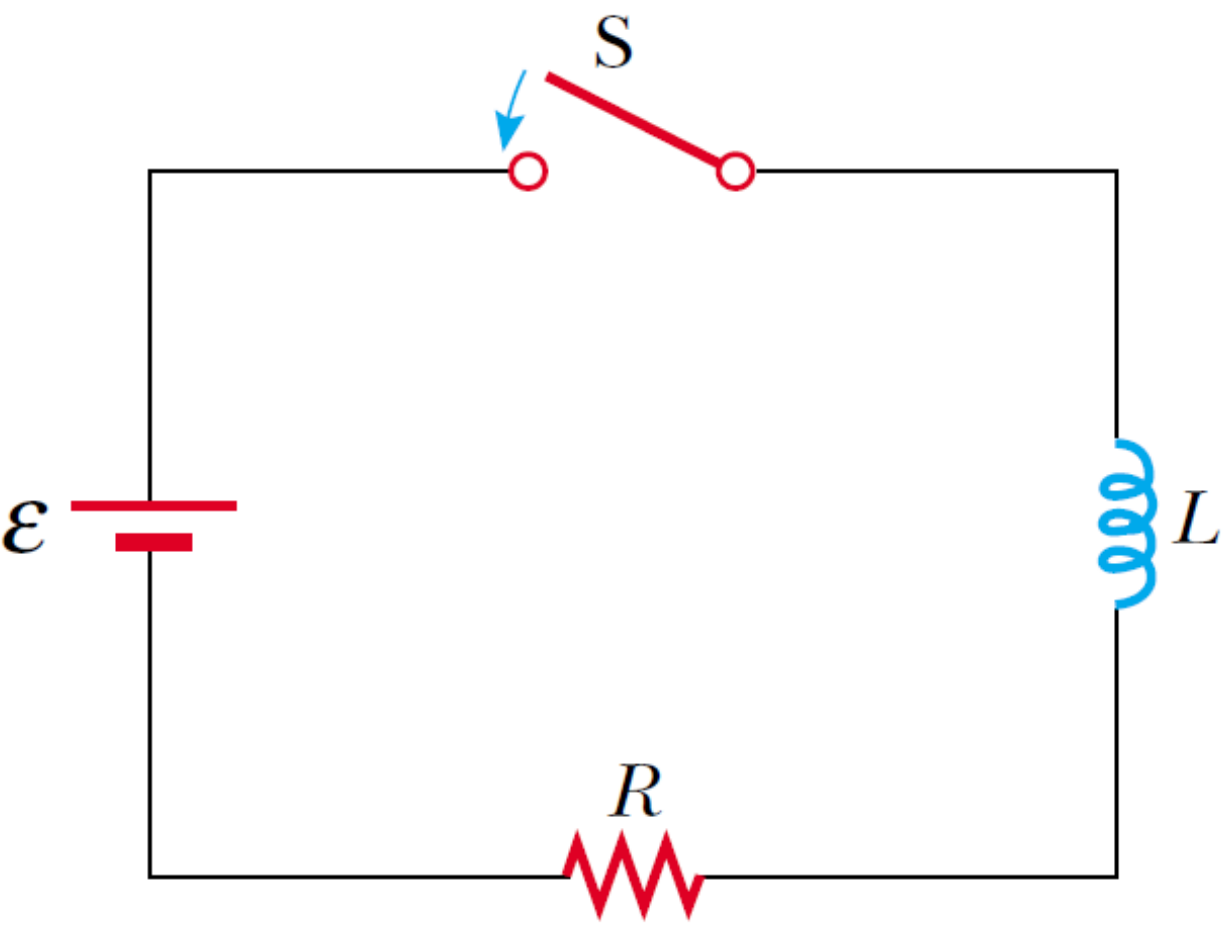
\includegraphics[scale = 0.28]{oz07/resources/oef-1-opgave.png}
    \end{center}
\end{minipage}
\vspace{0.3cm}

% \begin{description}[labelwidth=1.5cm, leftmargin=!]
%     \item[Geg. :] 
%     \item[Gevr. :] 
%     \item[Opl. :]
% \end{description}

\begin{description}[labelwidth=1.5cm, leftmargin=!]
    \item[Geg. :] $ \mathcal{E} = 6,00 $ V, $ L = 8,00 $ mH, $ R = 4,00 \ \Omega $
\end{description}

\begin{enumerate}[(a)]
    \item 
        \begin{description}[labelwidth=1.5cm, leftmargin=!]
            \item[Gevr. :] $\tau$
            \item[Opl. :]
                De inductieve tijdsconstante $ \tau $ van het circuit is gelijk aan
                \begin{equation*}
                    \tau = \frac{L}{R} = \frac{8,00 \cdot 10^{-3}}{4,00} = 2 \cdot 10^{-3} \ \text{s}
                \end{equation*}
        \end{description}
    \item 
        \begin{description}[labelwidth=1.5cm, leftmargin=!]
            \item[Geg. :] $t_1 = 250 \ \mu$s
            \item[Gevr. :] $I(t_1)$
            \item[Opl. :]
                We passen de wet van Kirchhoff toe op het circuit
                \begin{equation*}
                    \mathcal{E} = L \frac{dI}{dt} + RI
                \end{equation*}
                wat een differentiaalvergelijking is met oplossing
                \begin{equation*}
                    I(t) = \frac{\mathcal{E}}{R} \left(1 - e^{\tfrac{-t}{\tau}} \right)
                \end{equation*}
                waarin we de gegeven waarde invullen
                \begin{equation*}
                    I(t_1) = 0.176 \ \text{A}.
                \end{equation*}

        \end{description}
    \item 
        \begin{description}[labelwidth=1.5cm, leftmargin=!]
            \item[Gevr. :] $\lim_{t\to\infty} I(t)$
            \item[Opl. :]
                De steady-state stroom is gelijk aan
                \begin{equation*}
                    \lim_{t\to\infty} I(t) = \frac{\mathcal{E}}{R}\left(1 - \lim_{t\to\infty} e^{\tfrac{-t}{\tau}}\right) = \frac{\mathcal{E}}{R} = 1.50 \ \text{A}.
                \end{equation*}
        \end{description}
    \item 
        \begin{description}[labelwidth=1.5cm, leftmargin=!]
            \item[Gevr. :] $t_{80\%}$
            \item[Opl. :]
                De maximale stroom, of de steady-state stroom, is gelijk aan
                \begin{equation*}
                    I_{max} = \frac{\mathcal{E}}{R} = 1.50 \ \text{A}.
                \end{equation*}
                De stroom $I_{80\%}$ wordt dus eigenlijk gegeven door
                \begin{equation*}
                    I_{80\%} = \left(1 - e^{\tfrac{-t_{80\%}}{\tau}}\right) I_{max}.
                \end{equation*}
                We zoeken nu de tijd $t_{80\%}$ waarvoor
                \begin{equation*}
                   e^{\tfrac{-t_{80\%}}{\tau}} = 0.20
                \end{equation*}
                wat uitkomt op 
                \begin{equation*}
                    t_{80\%} = -\tau \ln(0.20) = 3.22 \cdot 10^{-3}\ \text{s}.
                \end{equation*}
        \end{description}
\end{enumerate}

% \begin{description}[labelwidth=1.5cm, leftmargin=!]
%     \item[Geg. :]   $ \varepsilon = 6,00 $ V; $ L = 8,00 $ mH; $ R = 4,00 \ \Omega $;
% \end{description}

% \begin{enumerate}[(a)]
%     \item 
%         \begin{description}[labelwidth=1.5cm, leftmargin=!]
%             \item[Gevr. :]  $ \tau $;
%             \item[Opl. :]   $ \tau = \dfrac{L}{R} = \dfrac{8,00 \cdot 10^{-3}}{4,00} = 0,00200 $ s
%         \end{description}
%     \item 
%         \begin{description}[labelwidth=1.5cm, leftmargin=!]
%             \item[Gevr. :]  $ I_{250 \mu\textrm{s}} $;
%             \item[Opl. :]   $ I = I_{max} \cdot \left(1 - e^{-t/\tau} \right) $ 
            
%                             $ I_{max} = \dfrac{\varepsilon}{R} = \dfrac{6,00}{5,00} = 1,50 $ A
                            
%                             $ I = 1,50 \cdot \left(1 - e^{-500t} \right) $ 
                            
%                             $ I_{250 \mu\textrm{s}} = 1,50 \cdot \left(1 - e^{-500 \cdot 250 \cdot 10^{-6}} \right) 
%                             = 0,17625 $ A $ \approx 0,176 $ A
%         \end{description}
%     \item 
%         \begin{description}[labelwidth=1.5cm, leftmargin=!]
%             \item[Gevr. :]  $ I_{250 \mu\textrm{s}} $;
%             \item[Opl. :]   $ I_{ss} = \lim_{t \to +\infty}{I_{max} \cdot \left(1 - e^{-t/\tau} \right)} = I_{max} 
%                             = 1,50 $ A
%         \end{description}
%     \item 
%         \begin{description}[labelwidth=1.5cm, leftmargin=!]
%             \item[Gevr. :]  $ t_{80 \%} $;
%             \item[Opl. :]   $ I = 0,80 \cdot I_{max} $
            
%                             \hspace{-0.57cm} $ \Leftrightarrow 
%                             I_{max} \cdot \left(1 - e^{-t_{80 \%}/\tau} \right) = 0,80 \cdot I_{max} $
            
%                             \hspace{-0.57cm} $ \Leftrightarrow 
%                             1 - e^{-t_{80 \%}/\tau} = 0,80 $
            
%                             \hspace{-0.57cm} $ \Leftrightarrow 
%                             e^{-t_{80 \%}/\tau} = 0,20 $
            
%                             \hspace{-0.57cm} $ \Leftrightarrow 
%                             -t_{80 \%}/\tau = \ln{0,20} $
            
%                             \hspace{-0.57cm} $ \Leftrightarrow 
%                             t_{80 \%} = - \ln{0,20} \cdot \tau = - \ln{0,20} \cdot 0,00200 = 0,0032189 $ s $ \approx 3,22 $ ms
%         \end{description}
% \end{enumerate}

\vspace{1cm}